\section{Vorlesung}

\subsection{Variationsweite/Spannweite/Range}
\begin{equation*}
    V = x_{max} - x_{min}
\end{equation*}
Beispiel: höchster Wert: 10, niedrigster Wert 7 \\\textrightarrow 10 - 7 = 3 = IQR\\
Nachteil: Starke Abweichungen einzelner Werte können zu Fehlinterpretationen führen.

\subsection{Interquartilabstand/IQR}
\begin{equation*}
    IQR = Q_{0.75} - Q_{0.25}
\end{equation*}

\subsection{Varianz}
\textrightarrow durchschnittliche Abweichung, Voraussetuzung: Pseudometrisches Skalenniveau
\begin{align*}
    \sigma^{2}& = \frac{\sum_{i=1}^{n}(x_{i}-\overline{x})^2}{n}~~~\longleftarrow \textrm{Varianz für Grundgesamtheit}\\
    \textrm{s}^{2}& = \frac{\sum_{i=1}^{n}(x_{i}-\overline{x})^2}{n-1}~~~\longleftarrow \textrm{Varianz für Stichprobe}
\end{align*}

\subsection{Standardabweichung}
\begin{align*}
    \sigma^{2}& = \frac{\sum_{i=1}^{n}(x_{i}-\overline{x})^2}{n}~~~\longleftarrow \textrm{Varianz}\\
    \sqrt{\sigma^{2}}& = \sigma~~~\longleftarrow \textrm{Standartabweichung}
\end{align*}
\textbf{\underline{Beispiel:}}\hfill(von \href{https://de.statista.com/statistik/lexikon/definition/126/standardabweichung/#:~:text=Definition%20Standardabweichung,Auspr%C3%A4gungen%20eines%20Merkmals%20vom%20Durchschnitt.}{Statista})\\
Gefragt wurden 1.000 Personen, wie hoch ihre monatliche Handyrechnung ist. Der Mittelwert liegt bei 40 Euro und die Standardabweichung bei 27. Das heißt, dass die durchschnittliche Entfernung aller Antworten zum Mittelwert 27 Euro beträgt.\\
Man würde wiefolgt schreiben:
\begin{align*}
  \overline{x}&= 40\textrm{\EUR}\\
  \sigma&= 27\textrm{\EUR}\\
  \overline{x}&= 40\pm27\textrm{\EUR}
\end{align*}

\subsection{Übung}
Der IQR sind die mittleren 50\% der Verteilung.
\begin{figure}[h]
 \centering
 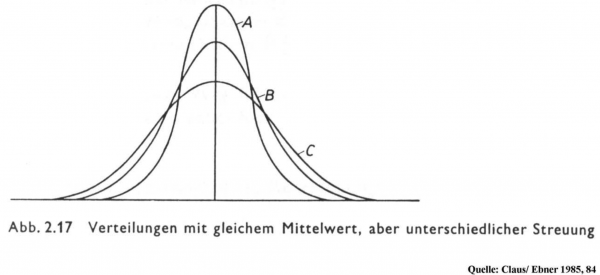
\includegraphics[scale=0.6]{./img/IQR_1.png}
 \caption{IQR}
\end{figure}
\vspace{0.5cm}
\begin{enumerate}
\item Ordne die IQRs der Verteilungen nach Größe. \solution{$IQR_{A} < IQR_{B} < IQR_{C}$}
\item Wie lautet die Standardabweichung und der Mittelwert für die folgenden Werte 44,67,102,42,52,42 \solution{circa 21,45}
\item Wie lautet die Standardabweichung für folgende Zahlen:\\
1,2,3,4,5 \solution{Varianz: 2; Standardabweichung: $\sqrt{2}$ }
\end{enumerate}
